\chapter{Pandas} \label{ch:pandas}

\section{Introduction to \texttt{pandas} Package}

The \verb|pandas| package is a widely used powerful data processing toolkit. With \verb|pandas|, Python gains the ability to handle data frames like Microsoft Excel. Some of the features and functions of \verb|pandas| are worth introducing separately before hand, hence this section.

This is not to say that other packages are less important or less complicated by all means. Some of these packages work together with \verb|pandas| to process data, while others may have their own ways to handle data frames. It is just that \verb|pandas| is a fundamental package that can be introduced stand alone.

Assume that \verb|pandas| is correctly installed in the machine, and a jupyter is opened as shown in Fig. \ref{ch:python:fig:jupyter_cover}.

\begin{figure}
	\centering
	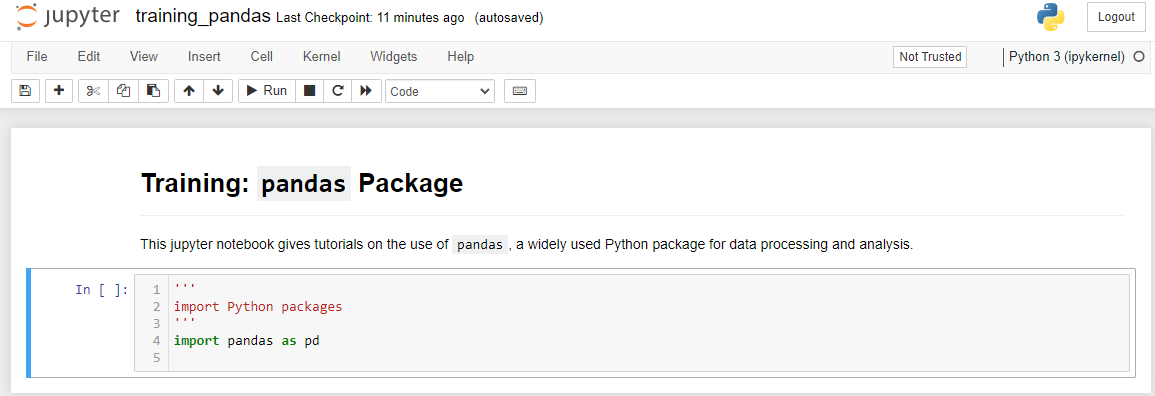
\includegraphics[width=350pt]{chapters/ch-python/figures/jupyter_cover.png}
	\caption{An example of a jupyter notebook.} \label{ch:python:fig:jupyter_cover}
\end{figure}


\section{Data Preprocessing}

Preprocessing of data is always required in data science. The format of data needs to be tidied, and error samples removed. Even with very clean input data, it is often necessary to do feature analysis and scaling (feature normalization). For verification of the effectiveness of the model to be built, data splitting into training set and testing set is often required.

Commonly used packages are imported as follows.
\begin{lstlisting}
import numpy as np
import matplotlib.pyplot as plt
import pandas as pd
\end{lstlisting}